
\chapter[Darstellung der Grundlagen \anmerkung{30-40 Seiten}]{Darstellung der Grundlagen\\
\normalsize{(nicht selbstgemachtes
Secondo,
MovingRegion,
T\o{}ssebro)}\anmerkung{30-40 Seiten}} \label{Kapitel2}
\minitoc
\newpage
\section{Secondo \anmerkung{10 Seiten}}
\anmerkung{Eine ausf"uhlichere Beschreibung von Secono, speziell des Konzeptes der Algebren, und eine Beschreibung der Algebren ,,Spatial-Algebra'' und ,Moving-Region-Algebra''.}
\subsection{Das Konzept der Secondo-Algebren}
\subsection{Spatial-Algebra}
\subsection{Moving-Region-Algebra}

\section{Das Paper von Erlend T\o{}ssebro \anmerkung{10 Seiten}}
\anmerkung{Hier beschreibe ich den Inhalt des Papers}

Eine der wichtigsten Grundlagen der vorliegenden Arbeit ist das Paper: ,,Creating Repesentations for Continuously Moving Regions from Observations'' \cite{TG} von Erlend T\o{}ssebro und Ralf Hartmund G"uting \cite{TG}, in dem die Autoren sich mit den theoretischen Grundlagen des Problems besch"aftigt, und L"osungsvorschl"age zu vielen der vorkommenden Teilprobleme gemacht haben.

\subsection{Matching-Strategien}\label{MatchSchwer}
In ihrem Paper nannten die Autoren drei verschiedene Matching-Strategien, die im folgenden kurz aufgef"uhrt werden:
\begin{enumerate}
\item Position of centroid

Bestimme den Schwerpunkt jedes Cycles,  bilde aus diesem einen gewichteten Graphen, mit den Entfernungen als Kantengewichte und suche in diesem "`N"achste Nachbarn"'.
\item Fixed threshold (set of cycles)

Matche zwei Cycles, wenn sie sich wechselseitig  mehr als threshold (in \%) "uberlappen.

\item Maximize Overlap (set of cycles)

Bilde einen gewichteten Graphen, in dem die Cycles Knoten sind, und dessen Kanten mit dem Grad der "Uberlappung gewichtet sind. Matche dann ein Cycle $c$ mit demjenigen, mit dem er die gr"o"ste "Uberlappung aufweist, und mit allen, f"ur die $c$ der Cycle mit der gr"o"sten "Uberlappung ist.
\end{enumerate} 

\section[Matching Shapes with a Reference Point]{Das Paper: ,,Matching Shapes with a Reference Point'' }\label{AARR}

Als eine sehr interessante Quelle erwieß sich das Paper \cite{AAR}, dessen Inhalt ich hier kurz wiedergeben möchte:

\subsection{Einleitung}

In ihrer Arbeit betrachten die Autoren Ähnlichkeiten von Objekten, die als Punktmengen repäsentiert werden. Diese Betrachtungen haben besondere Relevanz in Anwendungen der Mustererkennung. Als Maß für die Ähnlichkeit von zwei Objekten wird hier, wie auch in den meisten anderen Arbeiten zu diesen Themen, der Hausdorff-Abstand\index{Hausdorff-Abstand!als Norm} benutzt, den ich unter \ref{Hausdorff} näher beschreibe.

Um die Ähnlichkeit von zwei Objekten: $A$ und $B$ aus $\mathbb{R}^2$ oder aus $\mathbb{R}^3$ zu bestimmen, reicht es nicht den Hausdorff-Abstand $\delta_H(A,B)$ zu bestimmen, sondern man sucht die Abbildung $T\in\mathcal{T}$ unter der $\delta_H(A,T(B))$ minimal ist. $\mathcal{T}$ ist hierbei die Menge aller ,,erlaubten'' Abbildungen. Solche Abbildungen sind üblicherweise Rotationen, Verschiebungen, Skallierungen und Kombinationen aus solchen. Also sucht man:

$$\min_{T\in\mathcal{T}}\delta_H(A,T(B))$$

Die Suche nach dem optimalen $T$ ist im allgemeinen sehr kompliziert und aufwendig. Desshalb versuchen die Autoren keine optimale Abbildung $T_{OPT}$ zu finden, sondern sie suchen nach einer einfach und schnell berechenbaren Näherung, also einer Abbildung $T_{Approx}$, die $T_{OPT}$ zuverlässig und gut annähert.

\subsection{\index{Match!pseudooptimales}Das pseudooptimale Match}

Die Autoren definieren eine solche Abbildung als ,,pseudooptimales-Match mit Fehlerfaktor $\alpha$'' ( $\alpha\geq 1$, $\delta$ ist der optimale Hausdorff-Abstand)

$$\delta_H(A,T(B))\leq \alpha \delta$$

\subsection{\index{Referenzpunkt!Definition}Die Definition des Refenenzpunktes}

Der Versuch ein solches pseudo-optimales Matching zu finden unternehmen die Autoren über Referenzpunkte. Als $\mathcal{T}$ respektierenden Referenzpunkt definieren sie eine Abbildung $s:C_d\longrightarrow\mathbb{R}^d$, für die gilt:
$$\forall A, B\in C^d \text{ und } \forall T\in\mathcal{T}\Rightarrow$$
$$s(T(A))=T(s(A))\text{ (s ist äquivariant) und}$$
$$\exists c\geq0 \text{, so dass } \forall A, B \in C^d\Rightarrow$$
$$\Vert s(A)-s(B)\Vert\leq c\times\delta_H(A,B)\text{ (s ist Lipschitz-stetig mit Konstante c)}.$$

$c$ nennen die Autoren auch die Qualität von $s$.

\subsection{Algorithmen zum Finden von pseudooptimalen Lösungen}

Unter der Annahme, dass das ein solcher Referenzpunkt gefunden wurde, entwickeln die Autoren drei Algorithmen:
\begin{itemize}
\item Algorithmus $T$
\begin{enumerate}
\item Berechne $s(A)$ und $s(B)$.
\item Die pseudooptimale Lösung ist die Verschiebung um den Vektor $s(A)-s(B)$. Das Bild von $B$ nenne $B'$
\end{enumerate}

\item Algorithmus $R$
\begin{enumerate}
\item Wie in $T$.
\item Finde die optimale Rotation von $B'$ um $s(A)$. Diese Rotation, verknüpft mit der Verschiebung aus $T$, ist die pseudooptimale Lösung. Das Bild dieser nenne im Weiteren $B''$.

\end{enumerate}
\item Algorithmus $S$
\begin{enumerate}
\item Wie in $R$.
\item Bestimme die Durchmesser $d(A)$ und $d(B)$ und skalliere $B'$ um den Faktor $\alpha =\frac{d(A)}{d(B)}$.
\item Wie Schritt 2 in $R$ 
\end{enumerate}
\end{itemize}

Dann beweisen die Autoren:
\begin{enumerate}
\item Algorithmus $T$ findet eine pseudooptimale Abbildung für Verschiebungen. Der Verlustfaktor ist $\alpha=c+1$
\item Algorithmus $R$ findet eine pseudooptimale Abbildung für Kompositionen aus Verschiebungen und Rotationen.  Der Verlustfaktor ist $\alpha=c+1$
\item Algorithmus $S$ findet eine pseudooptimale Abbildung für Kompositionen aus Verschiebungen, Rotationen und Skallierungen. Der Verlustfaktor ist $\alpha=c+3$
\end{enumerate}

\subsection{\index{Referenzpunkt!SteinerPunkt}\index{Steinerpunkt!als Referenzpunkt}Die Wahl des richtigen Referenzpunktes}

Im weiteren Verlauf werden verschiedene Referenzpunkte untersucht. Der Schwerpunkt der konvexen Hüllen ist ein Referenzpunkt mit der Qualität $c=4\pi+3$. Der beste Referenzpunkt, den die Autoren finden konnten ist der Steinerpunkt, den ich in \ref{Steinerpunkt} beschreibe. Die Autoren zeigen, dass der Steinerpunkt ein Referenzpunkt für alle untersuchten Abbildungen ist und zeigen, dass dessen Qualität im zweidimensionalen $c=\frac{4}{\pi}$ ist. 

\subsection{Untere Schranke für die Qualitäten von Referenzpunkten}

Zuletzt finden die Autoren eine untere Schranke für die Qualität eines Referenzpunktes im Zweidimensionalen, unter Verschiebungen. Die Qualität eines Referenzpunktes unter diesen Abbildungen kann nicht besser sein als $\sqrt{\frac{4}{3}}$. Diese Behauptung wird bewiesen. 

Vergleicht man die Qualität des Steinerpunkts ($\frac{4}{\pi}\thickapprox 1,155$) mit diesem theoretischen minimalen Wert ($\sqrt{\frac{4}{3}}\thickapprox 1,27$), so stellt man fest, dass der Abstand der Qualitäten sehr gering ist. Der Steienerpunkt ist also warscheinlich der beste mögliche Referenzpunkt (für die Norm ,,Hausdorff-Abstand'').

\subsection{Die Bedeutung für meine Arbeit}\label{BedeutungAAR}

Zwar habe ich dieses Matching nicht so implementiert, wie es hier beschrieben wurde, ich habe aber ein Match programmiert, dass simultan zu dem Schwerpunkt-Match mit Schwellenwert von Herr T\o{}ssebro (siehe \ref{MatchSchwer}) funktioniert, nur dass hierbei der Schwerpunkt durch der Steinerpunkt ersetzt wird.

Betrachtet man sich den T\o{}ssebroschen Algorithmus, so stellt man fest, dass dieser starke Ähnlichkeit zu dem Algorithmus $R$ aus diesem Paper aufweist. Es steht also zu erwarten, dass dieser Algorithmus Matches finden wird, die gute Ergebnisse bezüglich des Hausdorff-Abstands liefern werden. Die hier beschriebenen Algorithmen konkret umzusetzen wäre eventuell eine gute Idee, die aber über den Umfang dieser Arbeit hinausgeht.

\section[Matching Shapes with Symmetric Difference]{Das Paper: ,,Matching Convex Shapes with Respect to Symmetric Difference'' }\label{AFRWW}
\anmerkung{Hier gebe ich eine Inhaltsangabe des Papers, und gehe speziell auf die Auswirkungen ein, die diese auf meine Matchingideen haben.}

Als eine weitere sehr interesannte Quelle erwies sich die Arbeit \cite{AFRW}, die stark auf der Anderen aufbaut. Auch von diesem Werk werde ich zunächst kurz den Inhalt wiedergeben.

\subsection{Die Grundlagen}

Zunächst klären die Autoren die Grundlagen dieser Arbeit. Da dieses Paper auf \cite{AAR} aufbaut, sind diese Grundlagen bereits aus dieser Arbeit bekannt. 

\subsection{\index{symmetrische Differenz!als Norm}Die symmetrische Differenz als Norm}

Als neue Norm für die Ähnlichkeit von zwei Objekten wird die \textbf{symmetrische Differenz} beschrieben. Diese ist unter  \ref{symDiff} näher beschrieben. Die Autoren machen darauf aufmerksam, dass diese Norm ein gutmütigeres Verhalten an den Tag legt, wenn die zu matchenden Polygone ,,gestört'' sind. Gestört soll in diesem Zusammenhang heißen, dass an sich an dem Rand des eigentlichen Polygon schmale, lange Dreiecke befinden. Unter \ref{symDiff} erläutere ich auch diesen Zusammenhang näher.

\subsection{\index{Schwerpunkt!als Referenzpunkt}\index{Referenzpunkt!Schwerpunkt}Der Schwerpunkt als Referenzpunkt für Verschiebungen}

Als Referenzpunkt für Abbildungen unter dieser Norm wird der Schwerpunkt der Polygone betrachtet. Dieser wird in dem Paper  nicht näher erläutert, ich beschreibe ihn trotzdem unter \ref{Schwerp}. 

Für $A, B \in \mathbb{R}^2$ und $\mathcal{T}$ die Menge der Verschiebungen wird der Satz

$$\delta_C (A,\tilde{T}(B))\leq\frac{11}{3}\min_{T\in\mathcal{T}}\delta_C(A,T(B))$$


aufgestellt und bewiesen. $\tilde{T}$ ist hierbei diejenige Verschiebung, die den Schwerpunkt von $B$ auf den Schwerpunkt von $A$ abbildet.

\subsection{allgemeinere Abbildungen}

Um diesen Referenzpunkt auch auf andere Abbildungen anwenden zu können, wird der Satz aufgestellt und bewiesen:

Gilt für eine Menge $\mathcal{T}$  von Abbildungen 
\begin{enumerate}
\item $s(T(A))=T(s(B))$ für $T\in\mathcal{T}$ und 
\item $\mathcal{T}$ ist abgeschlossen bezüglich der Kompsition von Abbildungen.
\end{enumerate}
dann ist der Schwerpunkt ein $\mathcal{T}$ respektierender Referenzpunkt mit Qualität $\frac{11}{3}$.

Abbildungen, die diese Bedingung erfüllen sind: 
\begin{itemize}
\item Kombinationen aus Verschiebungen und Rotationen,
\item Kombinationen aus Verschiebungen und Skallierungen,
\item Kombinationen aus allen drei Abbildungsarten und
\item belibige affine Abbildungen.
\end{itemize}

\subsection{Algorithmen zum Finden von pseudooptimalen Lösungen}

Nun erarbeiten die Autoren verschiedene Algorithmen, um Matchings für die verschiedenen Abbildungsarten durchführen zu können:
\begin{enumerate}
\item Verschiebungen

Verschiebt man $B$ um den Vektor $s(B)-s(A)$ auf $B'$, so hat man ein pseudooptimales Matching gefunden. Dieser Algorithmus entspricht dem Algorithmus $R$ aus dem letzten Abschnitt.

\item Kombinationen von Verschiebungen und Skallierungen

Verschiebt man zunächst $B$ wie oben angegeben, und skalliert dann $B'$ an dem Fixpunkt $s(A)$ um den Faktor $\lambda$, so hat man ein pseudooptimales Matching gefunden. $\lambda$ ist hierbei der Faktor, bei dem dem $\delta_C(A,\lambda B')$ minimal ist. Dieser Faktor kann in Linearzeit berechnet werden, wie die Autoren zeigen.

\item Kombinationen aus Verschiebungen und Rotationen

Auch hier wird zunächt $B'$ duch Verschiebung, wie oben, gebildet. Nun wird der Winkel $\varphi$ gesucht, für den $\delta_C(A,t_\varphi( B'))$ minimal ist. $t_\varphi$ sei die Rotations-Abbildung um den Punkt $s(A)$. Eine wirklich effiziente Lösung dieses Problems können die Autoren leider nicht geben, so dass man leider keinen effizienten Algorithmus für Abbildungen angeben kann, die Rotationen enthalten. 
\end{enumerate}

\subsection{Fazit}

Falls man die symmetrische Differenz als Norm benutzt, kann man  zusammenfassend sagen:
\begin{itemize}
\item Schwerpunkte sind Referenzpunkte für alle relevanten Abbildungen und
\item das Matching auf dieser Grundlage für alle Kombinationen aus Verschiebungen und Skallierungen ein pseudooptimales Matching mit der Qualität $\frac{11}{3}$ liefert. 
\end{itemize} 
\subsection{Die Bedeutung für meine Arbeit}\label{BedeutungAFRW}

Ein Matching, dass den Schwerpunkt als Referenzpunkt benutz hat, ist ebenso bereits in der Arbeit von Erlend T\o{}ssebro enthalten, wie auch ein Matching, dass die Überlappung, also das Inversse der symmetrischen Differenz, benutzt. Zwar sind dessen Algorthmen, wie auch bei der verhergegangenen Arbeit, nicht so ausgefeilt, wie die Algorithemen dieses Papers, aber nach der Lektüre dieser Arbeit kommt schon der Verdacht auf, dass die Resultate des Schwerpunkt-Matchings und die des Überlappungs-Matchings starke Ähnlichkeiten aufweisen werden. 

\section{Grundlagen der Paper}
In den oben beschriebenen Papern wurden einige wichtige, allgemeingültige Begriffe eingeführt. Die Definition dieser wichtigen Begriffe nehme ich erst an dieser Stelle vor, um das Nachschlagen zu erleichtern.

\subsection{\index{Hausdorff-Abstand!Definition und Berechnung}Hausdorff-Abstand}\label{Hausdorff} 

Seien $A$ und $B$ zwei kompakte Teilmengen des $\mathbb{R}^2$ und sei $\Vert\centerdot\Vert$ die Euklidische Norm.
Dann definieren wir eine Hilfsfunktion $ \widetilde{\delta_H}  $, den einseitige Hausdoff-Abstand, wie folgt:
\[ \widetilde{\delta_H}(A,B):=\max_{a\in A} \;\min_{b\in B} \Vert a-b \Vert\]
Der einseitige Hausdorff-Abstand von Polygon $A$ zu Polygon $B$ ist so definiert, dass er der Abstand des am weitesten entfernten Punktes aus $A$ zu dem im am n"achsten gelegenen Punkt aus $B$ ist.  Im weiteren Schritt wird der Hausdorff-Abstand wie folgt definiert: 
\[\delta_H:=\max\{\widetilde{\delta_H}(A,B),\widetilde{\delta_H}(B,A)\}.\]
\begin{figure}
	\centering
	\includegraphics[scale=.6]{Hausdorff.eps}
	\caption[Der Hausdorff-Abstand zweier Polygone]{Der Hausdorff-Abstand zweier Polygone (grün und blau) ist das Paar mit dem größten Abstand (rot) unter allen Paaren, wie beschrieben (schwarz).}
	\label{fig:HausdorffAbstand}
\end{figure}
Nimmt man also von zwei Polygonen zu jedem Punkt der einen Menge den nächsten Punkt der anderen Menge, und umgekehrt und sucht dann das Paar mit dem größten Abstan, so ist dieser der Hausdorff-Abstand.



\subsection{\index{symmetrische Differenz!Definition}Die symmetrische Differenz}\label{symDiff}
\begin{figure}
	\centering
	\includegraphics[scale=.6]{SymDiff.eps}
	\caption[Die symmetrische Differenz zweier Polygone]{Die symetriche Differenz der beiden Polygone aus dem Schaubild \ref{fig:HausdorffAbstand} ist der Flächeninhalt der roten Fläche.}
	\label{fig:SymDiffBild}
\end{figure}

In \cite{AFRW} wird vorgeschlagen den Fl"acheninhalt der symmetrischen Differenz als Abstands-Ma"s zweier konvexer Polygone zu benutzen. Die Symmetrische Differenz von zwei kompakten Teilmengen $A$ und $B$ des $\mathbb{R}^2 $ ist definiert als:
\[A\bigtriangleup B:=(A\setminus B)\cup(B\setminus A).\]
Wenn $A(\cdot)$ der Fl"acheninhalt ist, so bildet $\delta_S$ den Abstand nach der symmetrischen Differenz:
\[\delta_S:=A(A \bigtriangleup B).\]
in \cite{TG} schlagen die Autoren vor, die Überlappung $A\cap B$ als Maß für die Qualität eines Matchings zu benutzen. Wegen:
$$|A\bigtriangleup B|+|A\cap B|=|A\cup B|$$
ist klar, dass ein Match, dass die symmetrische Differenz minimiert,zu dem selben Ergebniss kommen wird, wie ein Match, dass die Überlappung maximiert.

In \cite{AFRW} wurde beschrieben, dass das Verhalten der symmetrischen Differenz relativ ,,gutmütig'' im Bezug auf gestörte Daten sei. Die Zeichnung \ref{fig:VergleichMetrik} erläutert diesen Zusammenhang. Die beiden Polygone sehen den Polygonen aus den Bildern \ref{fig:HausdorffAbstand} und \ref{fig:SymDiffBild} recht ähnlich, nur zwei Punke sind jedem Polygon ergäntzt worden. Dennoch ist der Hausdorf-Abstand um 100\% gestiegen, die Fläche der symmetrischen Differenz hingegen nur etwa um 8\%.

\begin{figure}
	\centering
	\includegraphics[scale=.6]{Metrikengestoert.eps}
	\caption{Hausdorff-Abstand und symmetrische Differenz im Vergleich}
	\label{fig:VergleichMetrik}
\end{figure}


\subsection{\index{Steinerpunkt!Definition}Der Steinerpunkt}\label{Steinerpunkt}

In \cite{Sch} wird der Steinerpunkt beschrieben "`als Schwerpunkt der Massenverteilung, die bei einem konvexen Polygon duch Belegung der Ecken mit den "au"seren Winkeln als Massen [...] gegeben ist"'. Folglich kann der Steiner-Punkt eines konvexen Polygones $P$, das aus den $n$ Eckpunkten $v_i$ besteht, berechnet werden ($\alpha_i$ ist hierbei der Innenwinkel von $v_i$) durch:
\[p_2(P)=\sum^n_{i=1}v_i (\pi-\alpha_i).\]
In der Zeichnung \ref{fig:Referenzpunkte} ist der Steienerpunkt grün eingezeichnet.


\subsection{\index{Schwerpunkt!Definition}Der Schwerpunkt}\label{Schwerp}

Der Schwerpunkt eines Polygones ist der Schwerpunkt der Massenverteilung, die entsteht, wenn man allen Eckpunkten die selbe Masse zuordnet. Er berechnet sich f"ur ein Polygon $P$ mit $n$ Eckpunkten $v_i$:
\[p_0(P)=\sum^n_{i=1}v_i \frac{1}{n}.\]
In der Zeichnung \ref{fig:Referenzpunkte} ist der Schwerpunkt mit roter Farbe markiert. 

Vergleicht man die beiden Referenzpunkte, so kann man sehen, dass der Schwerpunkt etwas ,,träger'' auf Punkte reagiert, die sich stark von den anderen unterscheiden (in dem dargestellten Beispiel der Punkt ganz rechts). In einem regelmäßigen n-Eck stimmen entsprechend beide Referenzpunkte überein. Vergleicht man dieses Verhalten der Referenzpunkt mit dem Verhalten der Normen für gestörte Werte (siehe Abbildung \ref{fig:VergleichMetrik}), so erscheint der Zusammenhang vom ,,empfindlicheren'' Hausdorff-Abstand und dem  Steinerpunkt, sowie der Zusammenhang zwischen den beiden ,,Gutmütigeren'' plausibel.

\begin{figure}
	\centering
	\includegraphics[scale=.8]{Referenzpunkte.eps}
	\caption[Vergleich beider Referenzpunkte]{Hier kann man beide Referenzpunkte im Vergleich sehen (der Schwerpunkt der Massenverteilung ist rot, der Steinerpunkt grün) }
	\label{fig:Referenzpunkte}
\end{figure}


%\printindex

